\newcommand{\red}{\leq_p}
\newcommand{\problem}[3]{
\begin{definition}
    {#1} \\
    \textbf{Input}: {#2}\\
    \textbf{Output}: {#3}
\end{definition}
}

\chapter{Preliminaries}\label{chapter:preliminaries}
\section{Isabelle and Dependencies}
\subsection*{Isabelle/HOL}
\textsc{Isabelle} is a generic interactive theorem prover. \textsc{HOL} is the Isabelle's formalization of Higher-Order Logic, a logical system with inductive sets, types , well-founded recursion etc. Our implementation requires the introduction of new datatypes, formalisation of natural numbers and integers. Thus, this type system is necessary.


\subsection*{HOL-Real\_Asymp and Laudau\_Symbols}
TODO

\subsection*{NREST}
TODO

\subsection*{The Karp21 Project}
The project aims to formalise all of the 21 \NPH\ problems in Karp's paper in 1972. Up till now, there are \textbf{TOCOUNT} problems of them finished, with a few other \NPH\ problems that are related but not in Karp's list. Our work also contributes to this project, formalising six of the remaining problems. Though dependent on this project, our work only reuses a few definitions by the predecessors, while the most formalisation and verification is original. An overview of the project is given in the following graph.
\begin{figure}[h!]
\centering
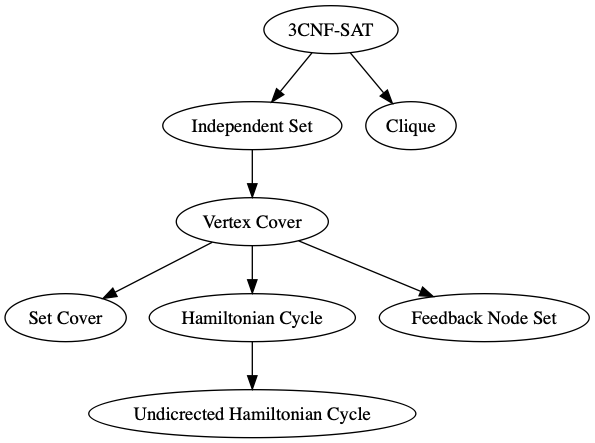
\includegraphics[scale=0.4]{figures/reductions.png}
\caption{Name}
\end{figure}

\subsection*{DigitsInBase}
This entry of Archive of Formal Proofs shows the uniqueness of representation of natural numbers given an arbitrary base. In other words, it proves the well-definedness of the n-ary counting systems. Our implementation benefits from this repository in showing the correctness of the polynomial reduction from \XC\ to \Part.

\section{NP-Hardness and polynomial reductions}
\subsection{Asymptotic Notation}
Conventionally, the asymptotic notation is used for defining complexity classes and for performing the algorithm analysis. 
We follow this convention and choose the big $\mathcal{O}$ notation for algorithm analysis. To begin with, we present a brief
introduction to the asymptotic notation.
\begin{definition}
    Let $f: \mathbb{R} \rightarrow \mathbb{R}$, $g: \mathbb{R} \rightarrow \mathbb{R}$ be two real valued functions with the same domain. 
    $f(x)$ is big $\mathcal{O}$ of $g(x)$, which writes
    \begin{align*}
        f(x) \in \mathcal{O}(g(x))
    \end{align*}
    if there exists a real $M \geq 0$ and a real $x_0$ s.t. 
    \begin{align*}
        |f(x)| \leq M |g(x)|, \forall x \geq x_0
    \end{align*}
\end{definition}
Thus, $f$ is above bounded by $g$. In other words, $f$ is utmost as complex as $g$. Following this definition 
we can derive many complexity classes by $g$. A short list of commonly encountered complexity classes is given 
in table.
\begin{table}[H]
    \centering 
    \begin{tabular}{|| c | c | c ||}
        \hline 
        Name & Big $\mathcal{O}$ Notation & Algorithmic Examples \\ 
        \hline 
        Constant & $\mathcal{O}(1)$ & Parity check\\
        \hline 
        Logarithmic & $\mathcal{O}(\log n)$ & Binary search in a sorted array \\ 
        \hline 
        Linear & $\mathcal{O}(n)$ & Addition of integers \\
        \hline 
        Quasilinear & $\mathcal{O}(n\log n)$ & Merge-sort and heap-sort \\
        \hline 
        Polynomial & $\mathcal{O} (n^c), c \in \mathbb{N}$ & Matrix multiplication \\
        \hline 
        Factorial & $\mathcal{O} (n!)$ & Enumeration of partitions of a set\\
        \hline 
    \end{tabular}
    \caption{List of commonly encountered complexity classes.}
\end{table}

In most cases of this paper, we only consider the polynomial class, which contains the most classes listed above 
as subclasses except for the factorial class. For the purpose of simplicity, we did not 
formalise the theory of asymptotic classes and big $\mathcal{O}$ notation, but used the 
available \textsc{Isabelle} dependencies of \textbf{HOL-Real\_Asymp} and \textbf{Landau\_Symbols}.

\subsection{Decision problems}
\begin{definition}
    A decision problem is a yes-no question on an infinite set of fixed type of inputs.
\end{definition}
Generally, if we refer to a decision problem $A$, we are referring to the set of all inputs for which the answer to the yes-no question is yes. 
The handling of a decision problem usually involves two questions:
\begin{enumerate}
    \item Is there an algorithm, which computes the solution to this problem, terminating on all inputs?
    \item If the answer to the first question is yes, is this algorithm efficient?
\end{enumerate}
If the answer to the first question is yes for a problem, it is a decidable problem, otherwise it is non-decidable. 
We do not expect a yes or no answer for the second question, but would like to find 
the optimal complexity for the algorithm. While some problems are possible to computed in 
an optimal upperbound by a deterministic algorithm, there are also a few problems, for which 
no deterministic polynomial algorithm is found. We define them formally as \NP.
\begin{definition}
    If there is a non-deterministic algorithm 
    that decides the solution to the problem in polynomial time, it is in the complexity 
    class \NP. 
\end{definition}
\begin{definition}
If a problem is at least as complex as the most complex problems in \NP. It is 
    in the complexity class \NPH.
\end{definition}

Although many attempts have benn made to prove or reject the existence of a non-deterministic algorithm 
for the \NP\ problems, our work focuses on the NP-Hardness. We would like to formally prove 
that many classical decision problems are \NPH. For this reason, we have to introduce polynomial reduction.

\subsection{Polynomial reductions}
Given two decision problems $A$ and $B$, 
a reduction is a function $f: A \rightarrow B$, 
which maps the inputs of the question of the first problem 
to that of the second problem. A reduction is polynomial 
if and only if the reduction function has a polynomial bound. 
For a polynomial reduction from $A$ to $B$, we writes $A \red B$. \\ \\
Let $M$ and $N$ denotes the domains of $A$ and $B$ respectively. 
A function $g: M \rightarrow N$ is a polynomial reduction 
if and only if the following conditions are fulfilled.
\begin{align}  
    &x \in A \iff g(x) \in B \\
    &\exists k\in \mathbb{N}. f \in \mathcal{O}(n^k)
\end{align}
For the convenience reason, we usually separate (2.1) into the soundness and completeness of the reduction.
\begin{align}
    soundness: \quad x \in A \Longrightarrow g(x) \in B \\
    completeness: \quad g(x) \in B \Longrightarrow x \in A
\end{align}

\subsection{NP-Hardness and \SAT}
To show a decision problem $B$ is \NPH, 
we have to find a \NPH\ problem and polynomial reduction 
s.t. $A \red B$. A first proven \NPH\ problem is \SAT, 
which was independently proven by Cook in 1971 and Levin in 1973. 
The \SAT\ problem is denoted by 
\problem{\SAT}{A propositional logical formula in 
conjunctive normal form. }{Is there a valid assignment for this formula?}
In the previous implementation of the project, the \SAT\ is defined by a list of clauses, with the clauses as the sets of variables.
There have been many attempts to solve \SAT\ problem in a polynomial bound, 
as well as many approaches to solve \SAT\ problem efficiently in certain scenarios.
Thus, \SAT\ is one of the most studies \NPH\ problems, from which there are also many \NPH\ problems reduced. 
Our first reduction also stems from \SAT, while all the other reductions are constructed upon novel introduced problems. 
More details on the reduction and implementation are given in Chapter 3 and Chapter 4. 
\begin{figure}
    \Snippet{cnf-sat-def}
    \caption{Definition of satisfiability problem in conjunctive normal form}
\end{figure}

\subsection*{Application of NREST and paradigms}
The NREST package offers an approach for approximating the complexity of non-deterministic processes.
This is especially useful when iterating a set, a collection or any other unordered data structures. Thus,
we use this package throughout this work. In our complexity analysis, the following commands are used. 
\begin{itemize}
    \item \textbf{$RETURNT$ res}. A command that returns the result \textbf{res}. It costs exactly one time unit.
    \item \textbf{$SPECT$ [cond $\rightarrow$ cost]}. A command used for checking a condition. Checking the condition \textbf{cond}
    take \textbf{cost} time units.
    \item \textbf{$SPEC$ $P$ $Q$}. A command used for assignment. Should $P\ x$ hold for an object $x$, it is a valid object after the assignment,
    which takes $Q\ x$ time units.
\end{itemize}
To apply the NREST approach in the complexity analysis, we convert the algorithm into the NREST commands as described above. Then we show 
that the complexity is above bounded in polynomial time. To clarify that the reduction is polynomial, we also show that the reduction
costs polynomial space. Thus, a paradigms of performing complexity analysis on reductions using NREST can be concluded.
\begin{enumerate}
    \item Proving that the reduction is correct.
    \item Implementing the reduction in NREST commands.
    \item Proving that the reduction costs polynomial time.
    \item Proving that the algorithm costs polynomial space.
\end{enumerate}
